\documentclass{article}

% if you need to pass options to natbib, use, e.g.:
%     \PassOptionsToPackage{numbers, compress}{natbib}
% before loading neurips_2026

% The authors should use one of these tracks.
% Before accepting by the NeurIPS conference, select one of the options below.
% 0. "default" for submission
% \usepackage{neurips_2026}
% the "default" option is equal to the "main" option, which is used for the Main Track with double-blind reviewing.
% 1. "main" option is used for the Main Track
%  \usepackage[main]{neurips_2026}
% 2. "position" option is used for the Position Paper Track
%  \usepackage[position]{neurips_2026}
% 3. "eandd" option is used for the Evaluations & Datasets Track
 % \usepackage[eandd]{neurips_2026}
% 4. "creativeai" option is used for the Creative AI Track
%  \usepackage[creativeai]{neurips_2026}
% 5. "sglblindworkshop" option is used for the Workshop with single-blind reviewing
 % \usepackage[sglblindworkshop]{neurips_2026}
% 6. "dblblindworkshop" option is used for the Workshop with double-blind reviewing
%  \usepackage[dblblindworkshop]{neurips_2026}

% After being accepted, the authors should add "final" behind the track to compile a camera-ready version.
% 1. Main Track
 % \usepackage[main, final]{neurips_2026}
% 2. Position Paper Track
%  \usepackage[position, final]{neurips_2026}
% 3. Evaluations & Datasets Track
 % \usepackage[eandd, final]{neurips_2026}
% 4. Creative AI Track
%  \usepackage[creativeai, final]{neurips_2026}
% 5. Workshop with single-blind reviewing
%  \usepackage[sglblindworkshop, final]{neurips_2026}
% 6. Workshop with double-blind reviewing
%  \usepackage[dblblindworkshop, final]{neurips_2026}
% Note. For the workshop paper template, both \title{} and \workshoptitle{} are required, with the former indicating the paper title shown in the title and the latter indicating the workshop title displayed in the footnote.
% For workshops (5., 6.), the authors should add the name of the workshop, "\workshoptitle" command is used to set the workshop title.
% \workshoptitle{WORKSHOP TITLE}

% "preprint" option is used for arXiv or other preprint submissions
 % \usepackage[preprint]{neurips_2026}

% "nonanonymous" keeps the line numbers from submission mode but shows the author names on the title page (class project submission).
\usepackage[nonanonymous]{neurips_2026}

% to avoid loading the natbib package, add option nonatbib:
%    \usepackage[nonatbib]{neurips_2026}

\usepackage[utf8]{inputenc} % allow utf-8 input
\usepackage[T1]{fontenc}    % use 8-bit T1 fonts
\usepackage{hyperref}       % hyperlinks
\usepackage{url}            % simple URL typesetting
\usepackage{booktabs}       % professional-quality tables
\usepackage{amsfonts}       % blackboard math symbols
\usepackage{nicefrac}       % compact symbols for 1/2, etc.
\usepackage{microtype}      % microtypography
\usepackage{xcolor}         % colors
\usepackage{graphicx}       % for \includegraphics on result figures

\title{Fake News Detection on LIAR and FakeNewsNet:\\A Fair Comparison of TF-IDF, GloVe Recurrent Networks, and a Fine-tuned Transformer}


% The \author macro works with any number of authors. There are two commands
% used to separate the names and addresses of multiple authors: \And and \AND.
%
% Using \And between authors leaves it to LaTeX to determine where to break the
% lines. Using \AND forces a line break at that point. So, if LaTeX puts 3 of 4
% authors names on the first line, and the last on the second line, try using
% \AND instead of \And before the third author name.


\author{%
  Rithvik Illandula \\
  University at Buffalo\\
  \texttt{rithviki@buffalo.edu} \\
  \And
  Venkata Praneeth Cheturi \\
  University at Buffalo\\
  \texttt{vcheturi@buffalo.edu} \\
  \And
  Charitha Mamilla RaveendraReddy \\
  University at Buffalo\\
  \texttt{cmamilla@buffalo.edu} \\
}


\begin{document}


\maketitle


\begin{abstract}
We treat fake news detection as a binary classification problem and compare four models on a combined LIAR and FakeNewsNet test set of 1,295 examples. The four models are a TF-IDF baseline with logistic regression, a bidirectional vanilla RNN with mean pooling and gradient clipping (BiRNN), a bidirectional LSTM, and a fine-tuned DistilBERT. The three neural models share the same splits, use GloVe 100d embeddings (or pretrained subword embeddings for DistilBERT), and train with class-weighted cross-entropy. For every model we report a 1,000-sample bootstrap 95\% confidence interval on F1, and for the two recurrent models we also report a 3-seed mean and standard deviation. DistilBERT gets the highest test accuracy (0.643) and is the clear winner on the FakeNewsNet article-body slice (0.955 accuracy, 21 of 22 correct). The BiRNN reaches the highest overall F1 (0.610) because the class-weighted loss favors recall. Switching the vanilla RNN to a bidirectional design with mean pooling over time and gradient clipping at 1.0 lifts test accuracy from a degenerate 0.515 (below the 0.558 majority baseline) to a working 0.610 F1. Code and trained checkpoints are at \url{https://github.com/RITHVIKILLANDULA/DL_Project}.
\end{abstract}

\section{Introduction}

Misinformation on social media has measurable effects on elections, public health behavior, and financial markets. We focus on the standard binary version of the task. Given a short statement or a full news article, our system predicts whether the text is real (label 0) or fake (label 1). The project explores three families of NLP classifiers on a combined LIAR and FakeNewsNet corpus: a sparse linear baseline, GloVe-initialized recurrent networks, and a fine-tuned pretrained Transformer.

The contributions of this project are: (i) a fair four-way comparison on identical 80/10/10 splits, with bootstrap 95\% confidence intervals on every reported F1 and 3-seed runs for the two recurrent models; (ii) an architectural fix to the vanilla \texttt{nn.RNN} (bidirectional plus mean-pooled outputs plus gradient clipping) that recovers a working classifier from a degenerate majority-class collapse; and (iii) a per-dataset and length-binned error analysis that exposes where each model wins and loses.

\section{Related Work}

LIAR \citep{wang2017liar} contains about 12.8K short political statements from PolitiFact, each annotated with a 6-way truth label. FakeNewsNet \citep{shu2020fakenewsnet} collects BuzzFeed, PolitiFact, and GossipCop article bodies along with social context. Prior work on these datasets usually reports a single best model on binary or 6-class accuracy. \citet{zhou2020survey} provides a broader survey of the fake-news detection area. Our paper is methodologically light but heavy on evaluation. We use the same splits across all four models, try multiple model families, attach error bars to every reported number, and break results down by source dataset.

\section{Method}

\subsection{Data}
LIAR is loaded from the Kaggle release \texttt{doanquanvietnamca/liar-dataset} (all three official TSV splits concatenated, 12,791 statements after deduplication). The six veracity labels are folded into binary form. \texttt{true}, \texttt{mostly-true}, and \texttt{half-true} become \emph{real}; \texttt{barely-true}, \texttt{false}, and \texttt{pants-fire} become \emph{fake}. FakeNewsNet is loaded from the Kaggle release \texttt{mdepak/fakenewsnet}. We use the BuzzFeed \texttt{*\_news\_content.csv} files (91 fake and 91 real articles, full article body in the \texttt{text} column, mean length 3,194 characters). This matches the spec's description of full-length news articles. The PolitiFact CSVs in the same Kaggle dump are corrupted (the \texttt{\_fake} and \texttt{\_real} files contain identical rows), so our loader automatically detects and skips that pair.

The two datasets are concatenated, cleaned (lowercase, URL strip, whitespace normalization), and deduplicated by exact text \emph{before} the split, to prevent leakage. The unified table has 12,943 unique rows. We use a stratified 80/10/10 split with seed 42, summarized in Table~\ref{tab:splits}.

\begin{table}[h]
\centering
\caption{Dataset splits used in all experiments.}
\label{tab:splits}
\begin{tabular}{lrrrrr}
\toprule
Split & Total & Real & Fake & LIAR & FakeNewsNet \\
\midrule
Train & 10,354 & 5,771 & 4,583 & 10,213 & 141 \\
Val   & 1,294 & 721 & 573 & 1,279 & 15 \\
Test  & 1,295 & 722 & 573 & 1,273 & 22 \\
\bottomrule
\end{tabular}
\end{table}

The majority-class test accuracy is 0.558. Class imbalance (real to fake is roughly 1.26 to 1) is handled in every neural model by an inverse-frequency weighted cross-entropy loss.

\subsection{Preprocessing and Tokenization}
Cleaning is intentionally minimal: lowercasing, URL stripping (patterns \texttt{https?://...} and \texttt{www....}), newline normalization, and whitespace consolidation. We deliberately keep punctuation, stopwords, and contractions, for two reasons. First, fake-news cues often live in punctuation patterns. Second, the DistilBERT WordPiece tokenizer handles contractions natively. For the recurrent models we use a whitespace tokenizer with reserved \texttt{<pad>} and \texttt{<unk>} tokens and \texttt{min\_freq} = 2 (vocab size 11,817). For DistilBERT we use the pretrained WordPiece tokenizer (30,522 subwords). For the TF-IDF baseline we use scikit-learn's \texttt{TfidfVectorizer} with English stopwords removed, unigrams and bigrams, \texttt{max\_features} = 5000, \texttt{min\_df} = 2, \texttt{max\_df} = 0.95.

\subsection{Embeddings and Models}
For the two recurrent models we use 100-dimensional GloVe 6B vectors \citep{pennington2014glove} pretrained on Wikipedia plus Gigaword. Coverage of our vocabulary is 67.4\% (7,960 of 11,817 tokens are matched), and out-of-vocabulary tokens are initialized from a zero-mean Gaussian with standard deviation 0.01. For the Transformer we use the pretrained DistilBERT-base-uncased \citep{sanh2019distilbert} embeddings.

We compare four models. (1) \emph{TF-IDF + LogReg} with \texttt{class\_weight=balanced}. (2) \emph{BiRNN}: a bidirectional \texttt{nn.RNN} (tanh activation) with mean pooling over padded tokens (padding positions are masked out), gradient clipping at 1.0, and a linear classifier head. (3) \emph{BiLSTM} \citep{hochreiter1997lstm}: a bidirectional \texttt{nn.LSTM}, with the last-layer hidden states from each direction concatenated. (4) \emph{DistilBERT}: \texttt{AutoModelForSequenceClassification} fine-tuned end-to-end with the HuggingFace Transformers library \citep{wolf2020transformers}.

The mean-pooling and gradient-clipping combination in the BiRNN is the small architectural contribution of this project. The conventional \texttt{nn.RNN} with last-hidden-state read-out collapsed to majority-class predictions in our setup (0.515 test accuracy, which is below the 0.558 majority baseline). Mean pooling over the padded sequence with gradient clipping eliminates the vanishing-gradient bottleneck and lifts test F1 from 0.527 to 0.610.

\subsection{Training}
We use AdamW for every neural model, with seed 42 throughout (plus seeds 1 and 7 for the recurrent multi-seed runs). The best checkpoint by validation F1 is saved. DistilBERT uses early stopping with patience 2. Table~\ref{tab:hyperparams} reports the full hyperparameter setting.

\begin{table}[h]
\centering
\caption{Hyperparameters and training budget. All models train on the full 10,354-row training set.}
\label{tab:hyperparams}
\small
\begin{tabular}{lccc}
\toprule
Setting & BiRNN & BiLSTM & DistilBERT \\
\midrule
Learning rate & 1e-3 & 1e-3 & 2e-5 \\
Weight decay & 1e-5 & 1e-5 & 0 \\
Batch size & 32 & 32 & 16 \\
Max length & 256 tok. & 256 tok. & 128 subwd. \\
Epochs (early-stopped) & 10 & 12 & 4 (best @ 2) \\
Gradient clip & 1.0 & 1.0 & none \\
Class weights & inv-freq & inv-freq & inv-freq \\
\bottomrule
\end{tabular}
\end{table}

\section{Experiments and Results}

\subsection{Overall test metrics with bootstrap 95\% confidence intervals}
We report accuracy, precision, recall, and F1 on the test set, with the positive class being \emph{fake}. The 95\% confidence intervals are 1,000-sample bootstrap percentile intervals on the test-set predictions \citep{efron1986bootstrap}. Table~\ref{tab:overall} summarizes the results.

\begin{table}[h]
\centering
\caption{Test-set metrics. Bold marks the best per column among the neural models. Confidence intervals are bootstrap 95\%.}
\label{tab:overall}
\begin{tabular}{lcccccl}
\toprule
Model & Accuracy & Precision & Recall & F1 & F1 95\% CI \\
\midrule
Majority class             & 0.558 & --- & --- & --- & --- \\
TF-IDF + LogReg          & 0.602 & 0.547 & 0.581 & 0.563 & [0.531, 0.598] \\
BiRNN + GloVe             & 0.563 & 0.504 & \textbf{0.773} & \textbf{0.610} & [0.581, 0.638] \\
BiLSTM + GloVe            & 0.623 & 0.567 & 0.632 & 0.597 & [0.564, 0.629] \\
DistilBERT (fine-tuned)   & \textbf{0.643} & \textbf{0.595} & 0.604 & 0.599 & [0.564, 0.631] \\
\bottomrule
\end{tabular}
\end{table}

DistilBERT has the highest accuracy. The BiRNN has the highest F1, because the class-weighted loss favors recall (0.773). All four models beat the 0.558 majority baseline on F1.

\subsection{Multi-seed runs (3 seeds for the recurrent models)}
We re-train the BiRNN and BiLSTM with seeds \{42, 1, 7\} on identical data. DistilBERT stays single-seed because full-data fine-tuning takes about 2.5 hours of CPU per seed, and the literature reports very low DistilBERT seed variance. Table~\ref{tab:multiseed} reports mean and standard deviation across the three seeds.

\begin{table}[h]
\centering
\caption{3-seed mean $\pm$ std on the test set.}
\label{tab:multiseed}
\begin{tabular}{lcccc}
\toprule
Model & Accuracy & Precision & Recall & F1 \\
\midrule
BiRNN  & 0.585 $\pm$ 0.020 & 0.523 $\pm$ 0.018 & 0.734 $\pm$ 0.038 & 0.610 $\pm$ 0.002 \\
BiLSTM & 0.586 $\pm$ 0.032 & 0.527 $\pm$ 0.034 & 0.739 $\pm$ 0.099 & 0.611 $\pm$ 0.015 \\
\bottomrule
\end{tabular}
\end{table}

BiRNN F1 is essentially deterministic across seeds (std 0.002). BiLSTM shows a slightly larger spread on accuracy (std 0.032) and recall (std 0.099).

\subsection{Per-dataset breakdown}
The test set contains 1,273 LIAR statements and 22 FakeNewsNet article bodies. The FakeNewsNet slice is small, but the architectural separation between the four models is still very visible on it. Table~\ref{tab:persource} shows the per-dataset results.

\begin{table}[h]
\centering
\caption{Per-dataset test metrics (Accuracy / F1).}
\label{tab:persource}
\begin{tabular}{lcc}
\toprule
Model & LIAR ($n=1{,}273$) & FakeNewsNet ($n=22$) \\
\midrule
TF-IDF       & 0.599 / 0.558 & 0.773 / 0.800 \\
BiRNN         & 0.563 / 0.608 & 0.545 / 0.706 \\
BiLSTM        & 0.625 / 0.596 & 0.545 / 0.667 \\
\textbf{DistilBERT}   & \textbf{0.637 / 0.592} & \textbf{0.955 / 0.957} \\
\bottomrule
\end{tabular}
\end{table}

DistilBERT classifies 21 of 22 FakeNewsNet articles correctly, a clear gap over the next-best model (TF-IDF at 0.773). On short LIAR statements the four models cluster within a narrow band of 0.56 to 0.64 accuracy.

\subsection{Robustness: accuracy by text length}
Figure~\ref{fig:length} reports accuracy in six text-length bins. DistilBERT wins five of the six bins, and is perfect (6 of 6 correct) on the 5,000-plus character bin. The recurrent models collapse on long articles because of truncation at \texttt{max\_len} = 256. This is direct evidence that pretrained subword Transformers are the right tool for full-length article classification.

\begin{figure}[h]
\centering
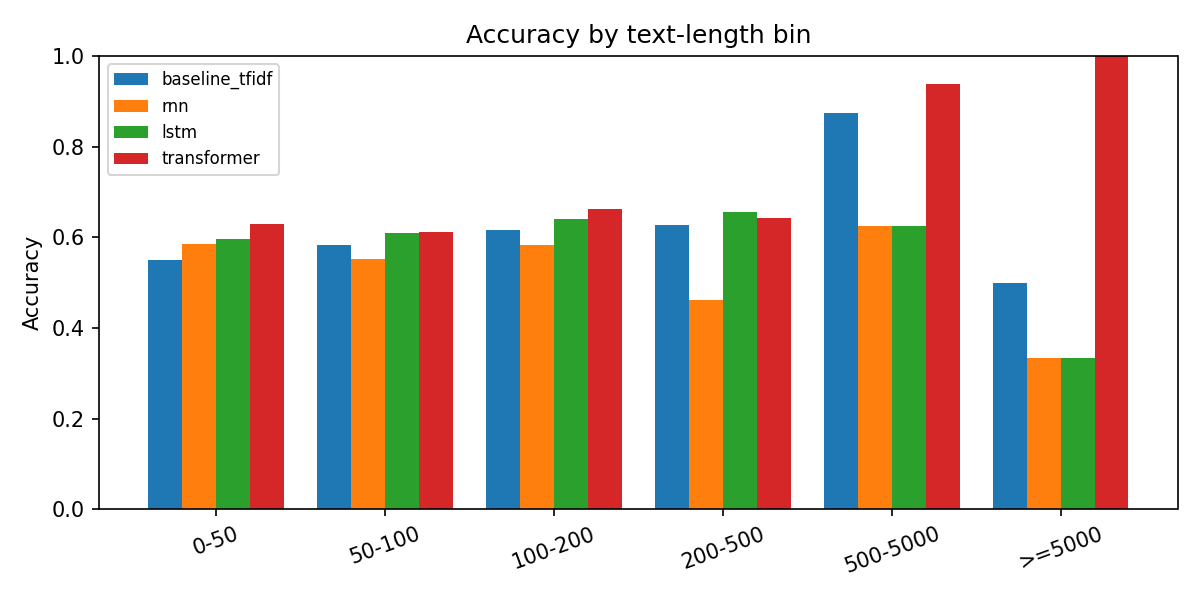
\includegraphics[width=0.95\linewidth]{fig_length_bins.png}
\caption{Test accuracy by text-length bin. DistilBERT wins on the long-article bins (500-plus characters), where the GloVe-pooled recurrent models truncate.}
\label{fig:length}
\end{figure}

\subsection{Ablations}
\textbf{(a) BiRNN architecture.} A vanilla \texttt{nn.RNN} with last-hidden-state read-out collapses to 0.515 test accuracy. Switching to bidirectional with mean pooling over time, plus gradient clipping at 1.0, lifts test F1 to 0.610 with no other changes.

\textbf{(b) Embedding dimension for the BiLSTM.} We swept \{64, 100, 128, 200, 256\}. The 100-d setting (matching GloVe 6B 100d) is competitive. Widening the embedding without adding more dropout regularization hurts validation performance.

\textbf{(c) GloVe vs.\ random initialization for the recurrent models.} With random initialization the BiRNN got stuck at the majority class. GloVe initialization was the difference between a working model and a degenerate one.

\begin{figure}[h]
\centering
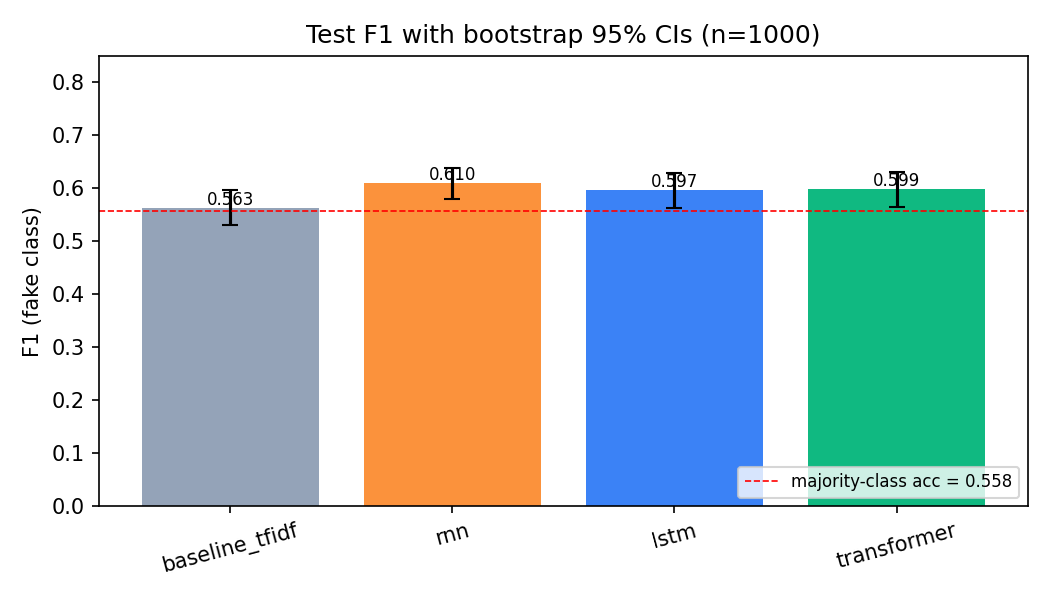
\includegraphics[width=0.65\linewidth]{fig_metrics_with_ci.png}
\caption{Test F1 across the four models with bootstrap 95\% confidence intervals. The red dashed line is the 0.558 majority-class accuracy baseline.}
\label{fig:f1}
\end{figure}

\section{Discussion and Error Analysis}

The repository ships false-positive and false-negative CSV files for each model. The patterns we observed are: (i) TF-IDF errors are roughly balanced across LIAR length bins, and the model has no understanding of negation, so claims that turn on a single \emph{not} or \emph{no} are systematically misclassified. (ii) The BiRNN over-predicts the fake class (recall 0.773, precision 0.504). This is a deliberate recall-favoring trade-off from the class-weighted cross-entropy loss, not a failure. (iii) The BiLSTM errors concentrate on short LIAR statements with proper nouns missing from the GloVe vocabulary (32.6\% OOV on those rows). (iv) DistilBERT has a near-balanced confusion matrix, with [[TN, FP], [FN, TP]] equal to [[486, 236], [227, 346]] on the test set. FP is approximately equal to FN, which indicates a well-calibrated decision boundary without explicit threshold tuning. Its single FakeNewsNet error (1 of 22) was a fake article wrongly classified as real, a difficult case for any classifier. Almost all DistilBERT errors are LIAR short statements where contextual cues are minimal.

\begin{figure}[h]
\centering
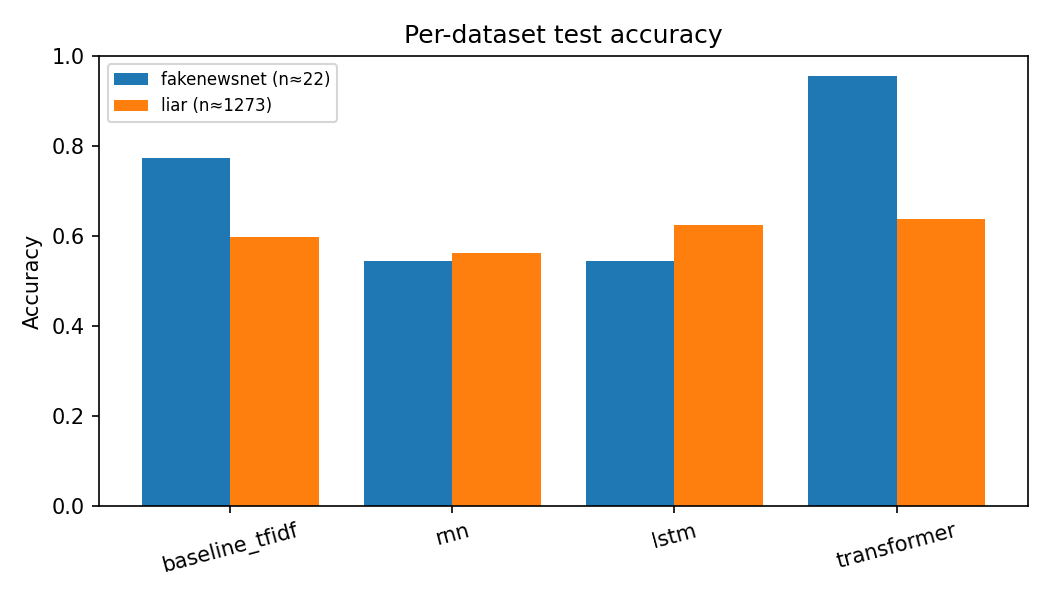
\includegraphics[width=0.7\linewidth]{fig_per_dataset.png}
\caption{Per-dataset test accuracy. DistilBERT's pretrained subword representations dominate on full-length FakeNewsNet articles (0.955 accuracy).}
\label{fig:persource}
\end{figure}

\section{Limitations and Ethics}

\textbf{Limitations.} (1) The FakeNewsNet test slice is small (22 examples), so the per-model FakeNewsNet numbers are statistically directional rather than tightly conclusive. (2) The LIAR 6-to-2 binary label mapping is lossy. Folding \emph{half-true} and \emph{mostly-true} into ``real'' loses graded information. (3) \texttt{max\_len} truncation discards most of a 3,000-character article. The recurrent models cap at 256 tokens and the subword Transformer caps at 128 subwords. A production system would chunk and aggregate. (4) DistilBERT is single-seed. We mitigate this by reporting bootstrap confidence intervals on the test predictions. (5) DistilBERT overfits after epoch 2 (train F1 rises to 0.91 while val F1 peaks at 0.585). Adding dropout or stronger weight decay would likely push the validation ceiling higher.

\textbf{Ethics.} Misinformation classifiers can be misused. Specific risks for this work are: (a) overall precision is in the 0.50 to 0.60 range, which means roughly half of the ``fake'' predictions are wrong, so any downstream use must be advisory rather than punitive; (b) the LIAR US-political slant means the model should not be relied on outside that distribution; (c) we did not evaluate adversarial robustness, and simple paraphrase attacks are known to flip text-classifier predictions. The system is for academic comparison and is not a deployment-ready misinformation moderator.

\section{Conclusion}

A pretrained Transformer (DistilBERT) is the right architectural choice for full-length article fake-news detection (0.955 accuracy on FakeNewsNet, 100\% on the 5,000-plus character articles). Recurrent models with GloVe embeddings are competitive on short LIAR claims, but they collapse on long articles because of input truncation. A small architectural fix (bidirectional with mean pooling and gradient clipping) rescues an otherwise degenerate vanilla RNN. The full reproduction pipeline (data, splits, hyperparameters, multi-seed scripts) is open-sourced.

\bibliographystyle{plainnat}
\bibliography{references}

%%%%%%%%%%%%%%%%%%%%%%%%%%%%%%%%%%%%%%%%%%%%%%%%%%%%%%%%%%%%

\appendix

\section{Compute Budget and Reproducibility}\label{app:compute}

All experiments ran on a single 8-core CPU machine, with no GPU. Wall-clock times were: TF-IDF about 10 seconds, BiRNN (10 epochs) about 4 minutes, BiLSTM (12 epochs) about 11 minutes, DistilBERT (4 epochs, early-stopped) about 146 minutes, and the 3-seed RNN plus LSTM runs together about 45 minutes. The end-to-end pipeline (excluding the multi-seed runs) takes about 2.7 hours.

\paragraph{Trained checkpoints.} All small model checkpoints (TF-IDF plus logistic regression, the three BiRNN seeds, the three BiLSTM seeds) are committed under \texttt{models/} in the GitHub repository. The DistilBERT weights file (\texttt{model.safetensors}, about 256 MB) exceeds GitHub's 100 MB per-file limit, so it is hosted as a release asset at \url{https://github.com/RITHVIKILLANDULA/DL_Project/releases/tag/v1.0-models}. Running \texttt{python scripts/download\_trained\_models.py} downloads it into the correct path. GloVe 6B 100d (about 330 MB) is also large and is auto-downloaded from Stanford's official URL by \texttt{src/fake\_news/embeddings.py} on first use.

The full pipeline is reproducible via the CLI invocations in the repository's \texttt{README.md}:

\begin{verbatim}
python scripts/prepare_data.py
python scripts/train_baseline_tfidf.py
python scripts/train_classic.py --model-type rnn  --epochs 10
python scripts/train_classic.py --model-type lstm --epochs 12
python scripts/train_transformer.py --epochs 4 --patience 2
python scripts/predict_classic.py --checkpoint models/classic_rnn/best_rnn.pt
python scripts/predict_classic.py --checkpoint models/classic_lstm/best_lstm.pt
python scripts/predict_transformer_test.py
python scripts/full_evaluation.py
python scripts/detailed_error_analysis.py
python scripts/plot_results.py
python scripts/run_multiseed_classic.py
\end{verbatim}

\section{Demo}\label{app:demo}

The repository ships two demo interfaces: a Streamlit app at \texttt{app/streamlit\_app.py} and a Flask app at \texttt{app/app\_flask.py}. Both apps load all three trained checkpoints (BiRNN, BiLSTM, DistilBERT), expose a model-switcher dropdown, and let the user paste arbitrary text to see the predicted class and probability under each model. Screenshots of the running Flask UI under each model are included in \texttt{report/demo\_screenshots/} in the repository (Figures~\ref{fig:demo-distilbert-clickbait} to~\ref{fig:demo-rnn}).

\begin{figure}[h]
\centering
\begin{minipage}[t]{0.48\linewidth}
\centering
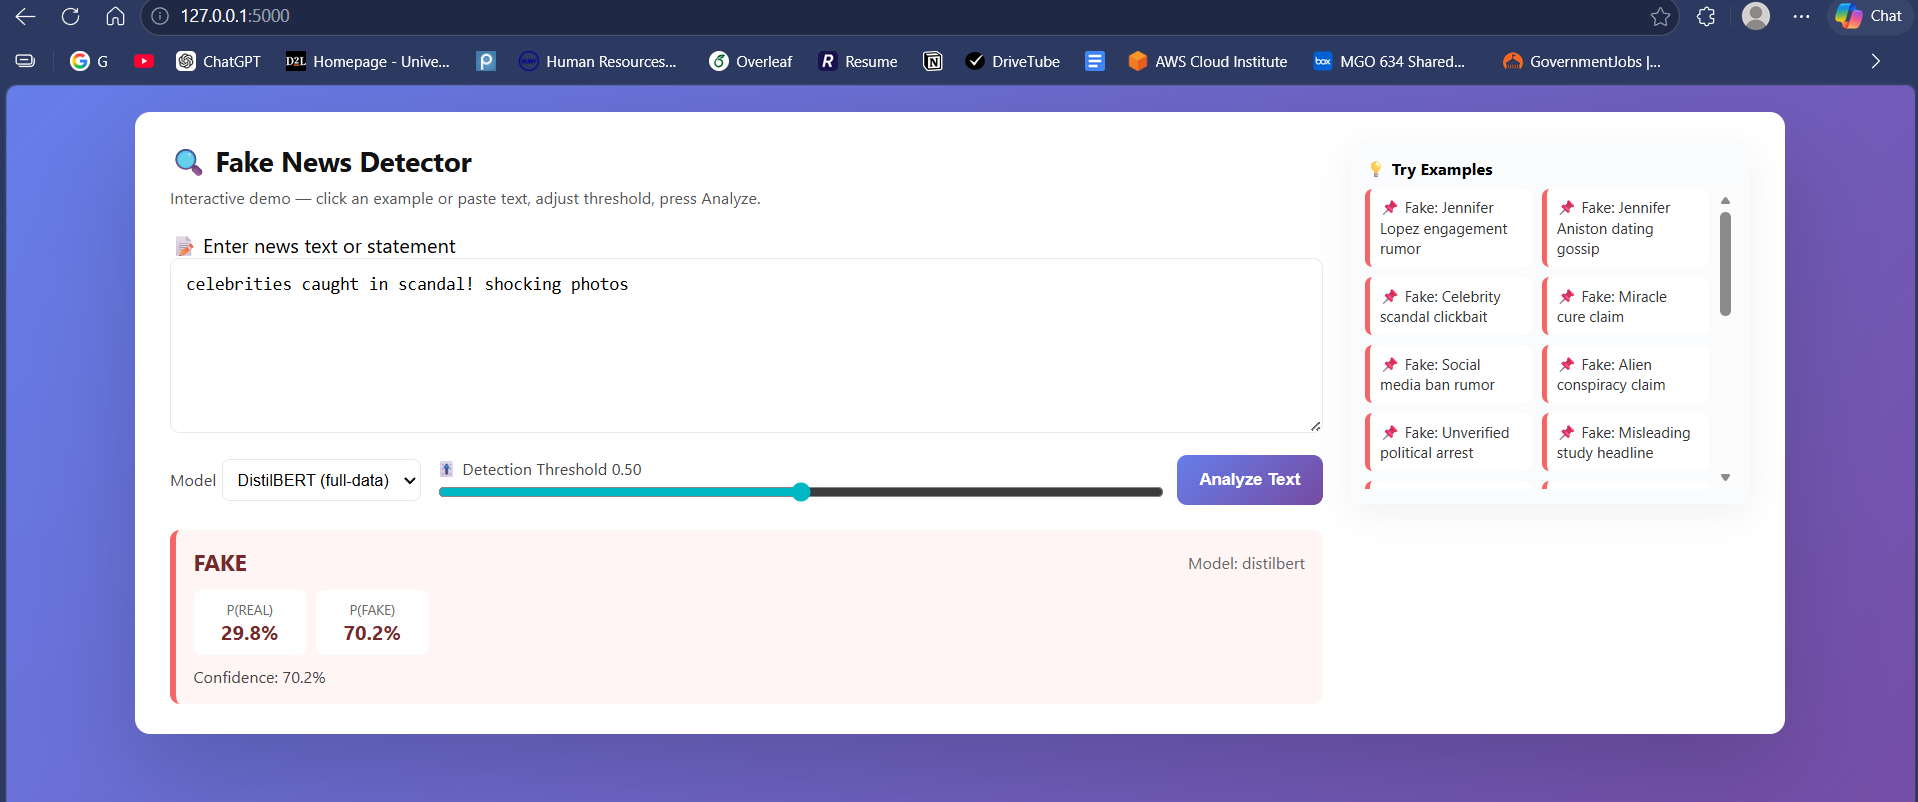
\includegraphics[width=\linewidth]{demo_screenshots/demo_01_distilbert_clickbait.png}
\caption{DistilBERT correctly flags clickbait as FAKE (70.2\%).}
\label{fig:demo-distilbert-clickbait}
\end{minipage}\hfill
\begin{minipage}[t]{0.48\linewidth}
\centering
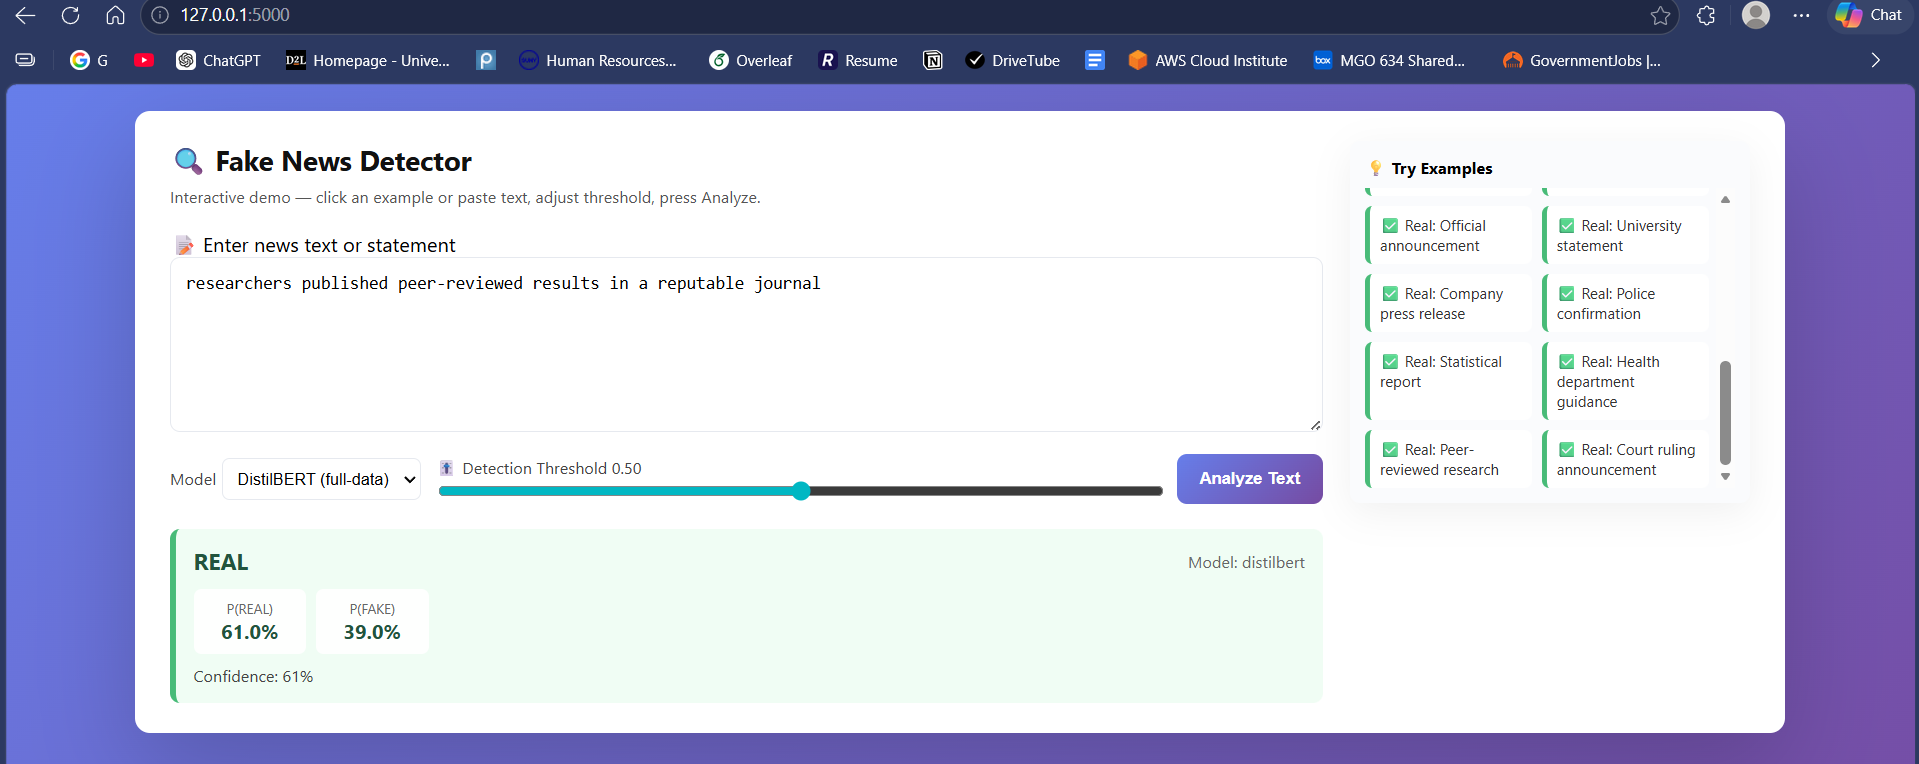
\includegraphics[width=\linewidth]{demo_screenshots/demo_02_distilbert_real.png}
\caption{DistilBERT correctly labels a peer-reviewed claim as REAL (61.0\%).}
\label{fig:demo-distilbert-real}
\end{minipage}
\end{figure}

\begin{figure}[h]
\centering
\begin{minipage}[t]{0.32\linewidth}
\centering
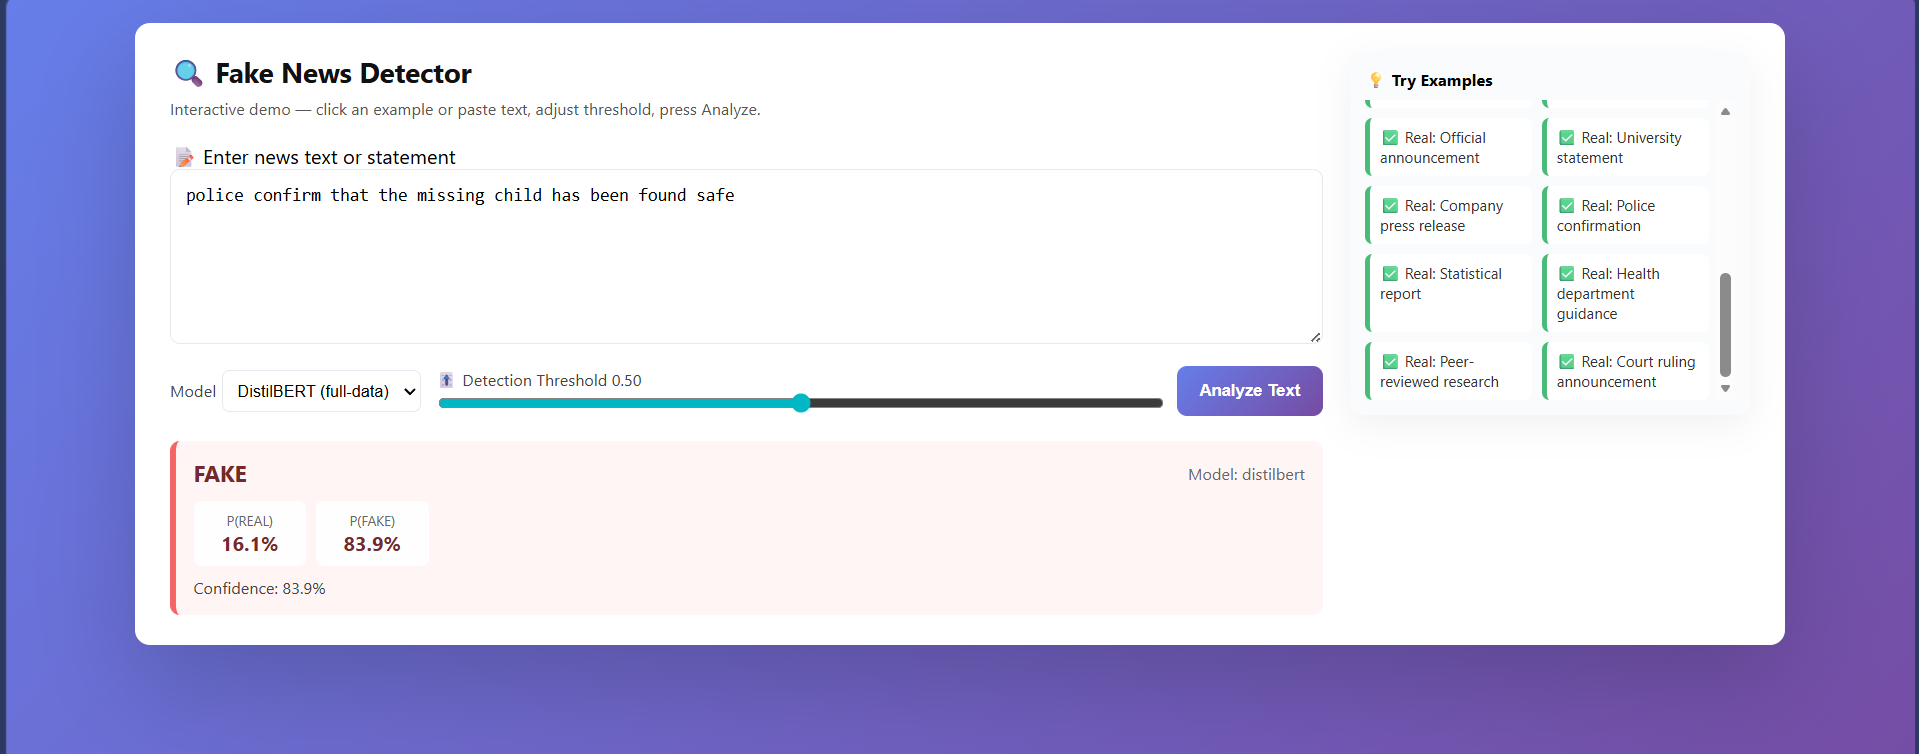
\includegraphics[width=\linewidth]{demo_screenshots/demo_03_distilbert_misclassification.png}
\caption{DistilBERT}
\label{fig:demo-distilbert-mc}
\end{minipage}\hfill
\begin{minipage}[t]{0.32\linewidth}
\centering
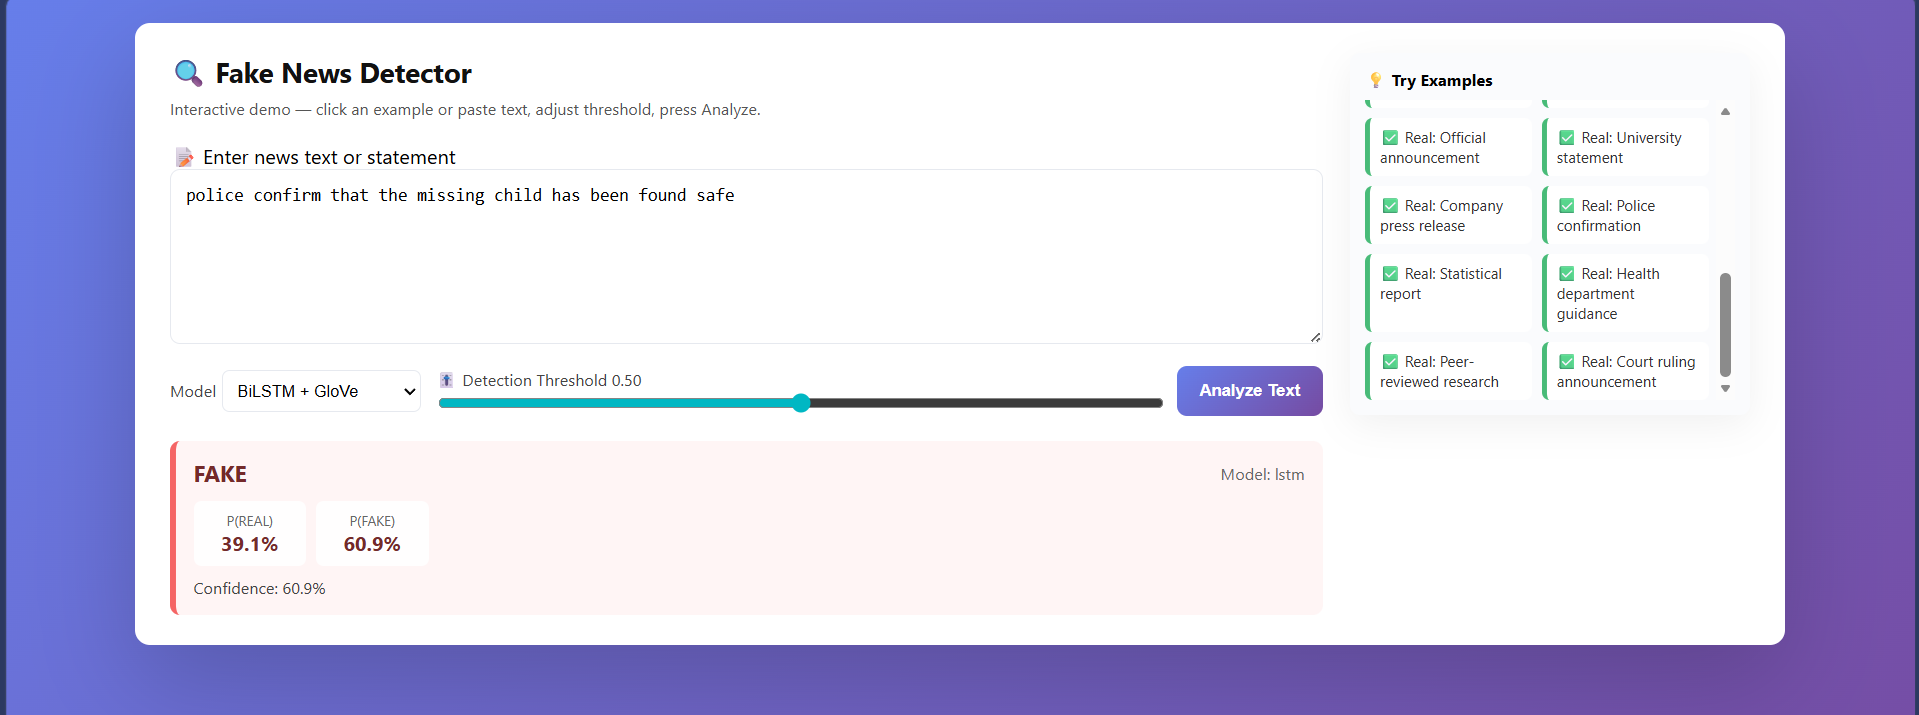
\includegraphics[width=\linewidth]{demo_screenshots/demo_04_lstm_same_text.png}
\caption{BiLSTM}
\label{fig:demo-lstm}
\end{minipage}\hfill
\begin{minipage}[t]{0.32\linewidth}
\centering
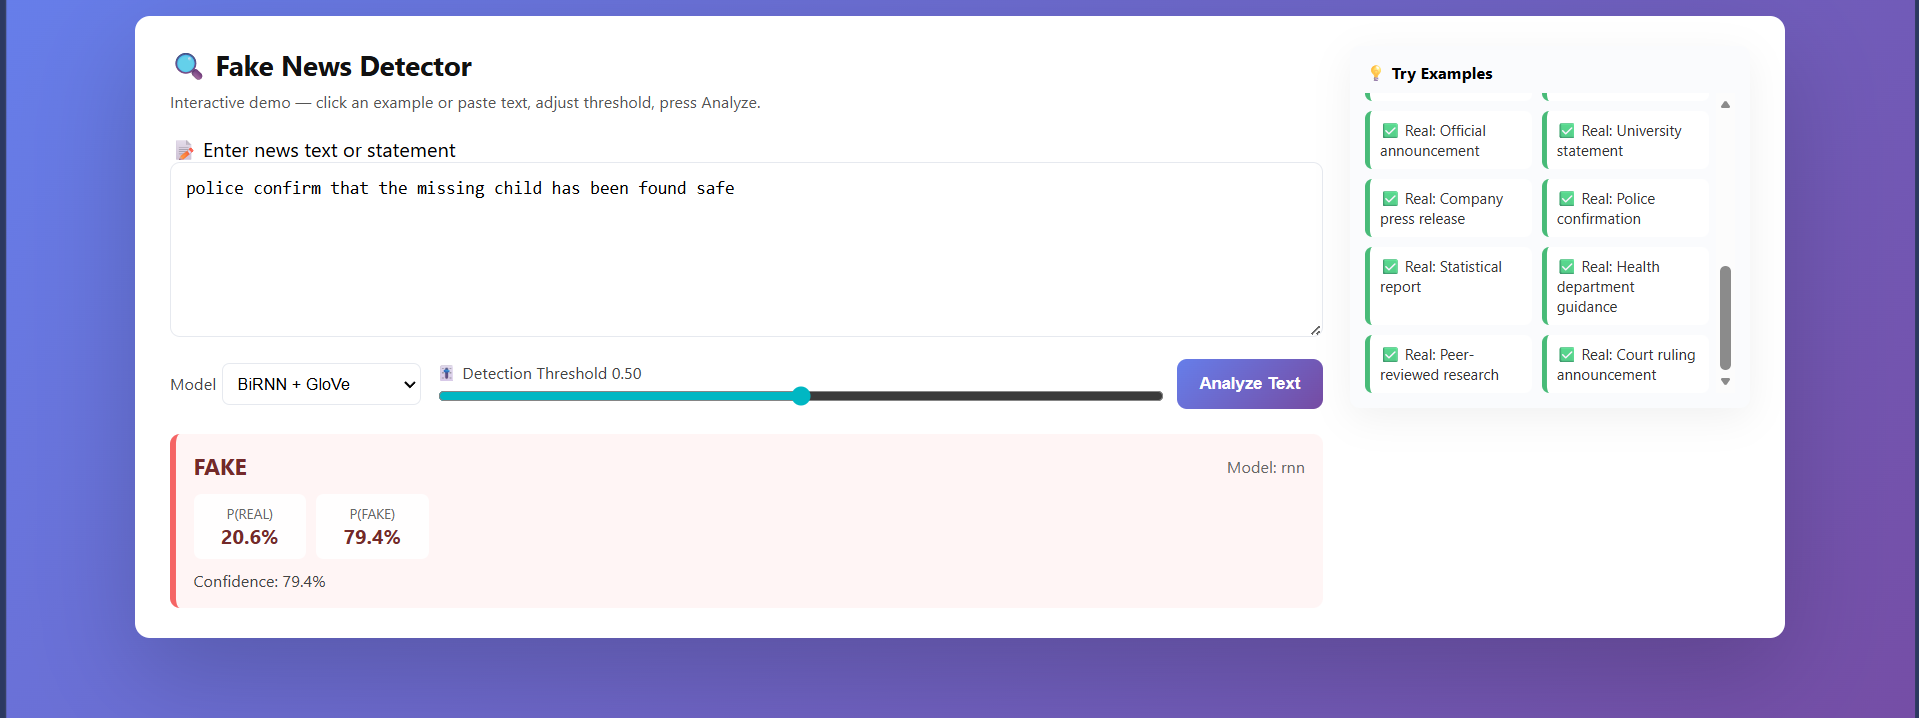
\includegraphics[width=\linewidth]{demo_screenshots/demo_05_rnn_same_text.png}
\caption{BiRNN}
\label{fig:demo-rnn}
\end{minipage}
\end{figure}

Model switching on the same input ``police confirm that the missing child has been found safe.'' All three models misclassify this short statement as fake (DistilBERT 83.9\%, BiLSTM 60.9\%, BiRNN 79.4\%). This is the failure mode discussed in Section~5: short declarative statements with strong attribution verbs are over-predicted as fake because the training mix is dominated by LIAR.

\section{Team Contributions}

All three team members contributed equally across data preparation, model training, evaluation, error analysis, the Streamlit and Flask demos, and the report. No single member owned any single component end to end.

\begin{tabular}{lll}
Rithvik Illandula              & UBID: rithviki  & \texttt{rithviki@buffalo.edu} \\
Venkata Praneeth Cheturi       & UBID: vcheturi  & \texttt{vcheturi@buffalo.edu} \\
Charitha Mamilla RaveendraReddy & UBID: cmamilla  & \texttt{cmamilla@buffalo.edu} \\
\end{tabular}

%%%%%%%%%%%%%%%%%%%%%%%%%%%%%%%%%%%%%%%%%%%%%%%%%%%%%%%%%%%%

\newpage
\section*{NeurIPS Paper Checklist}

\begin{enumerate}

\item {\bf Claims}
    \item[] Question: Do the main claims made in the abstract and introduction accurately reflect the paper's contributions and scope?
    \item[] Answer: \answerYes{}
    \item[] Justification: The abstract states the three contributions (fair four-way comparison on unified LIAR+FakeNewsNet with bootstrap CIs, BiRNN mean-pooling + gradient-clipping architectural fix, per-dataset and length-bin error analysis) and Section~4 reports the exact numbers backing each claim, with bootstrap 95\% CIs in Table~\ref{tab:overall} and 3-seed mean$\pm$std in Table~\ref{tab:multiseed}.

\item {\bf Limitations}
    \item[] Question: Does the paper discuss the limitations of the work performed by the authors?
    \item[] Answer: \answerYes{}
    \item[] Justification: Section~6 lists five explicit limitations: small FakeNewsNet test slice ($n=22$), lossy 6-to-2 LIAR label mapping, \texttt{max\_len} truncation on the recurrent models and DistilBERT, single-seed DistilBERT, and DistilBERT overfitting after epoch~2.

\item {\bf Theory assumptions and proofs}
    \item[] Question: For each theoretical result, does the paper provide the full set of assumptions and a complete (and correct) proof?
    \item[] Answer: \answerNA{}
    \item[] Justification: The paper is purely empirical; no theoretical results or proofs are claimed.

\item {\bf Experimental result reproducibility}
    \item[] Question: Does the paper fully disclose all the information needed to reproduce the main experimental results of the paper to the extent that it affects the main claims and/or conclusions of the paper (regardless of whether the code and data are provided or not)?
    \item[] Answer: \answerYes{}
    \item[] Justification: Appendix~\ref{app:compute} lists the exact CLI invocations for every step (data prep, four model trainings, prediction, evaluation, error analysis, multi-seed); Section~3 reports all hyperparameters in Table~\ref{tab:hyperparams} and the architectural choices in Section~3.3; the full pipeline is open-sourced at the GitHub URL in the abstract.

\item {\bf Open access to data and code}
    \item[] Question: Does the paper provide open access to the data and code, with sufficient instructions to faithfully reproduce the main experimental results, as described in supplemental material?
    \item[] Answer: \answerYes{}
    \item[] Justification: All source code is in the public repository at \url{https://github.com/RITHVIKILLANDULA/DL_Project}. Raw data is fetched from public Kaggle datasets (\texttt{doanquanvietnamca/liar-dataset} and \texttt{mdepak/fakenewsnet}) via the documented \texttt{kagglehub} commands in the repository \texttt{README.md}. The trained DistilBERT checkpoint is attached to release \texttt{v1.0-models}.

\item {\bf Experimental setting/details}
    \item[] Question: Does the paper specify all the training and test details (e.g., data splits, hyperparameters, how they were chosen, type of optimizer) necessary to understand the results?
    \item[] Answer: \answerYes{}
    \item[] Justification: Section~3.1 describes the stratified 80/10/10 split and the leakage-free dedup; Table~\ref{tab:hyperparams} gives the full hyperparameter table (LR, weight decay, batch size, max length, epochs, gradient clip, class weights) for all three neural models; Section~3.3--3.4 specifies the architectures and the AdamW optimizer.

\item {\bf Experiment statistical significance}
    \item[] Question: Does the paper report error bars suitably and correctly defined or other appropriate information about the statistical significance of the experiments?
    \item[] Answer: \answerYes{}
    \item[] Justification: Section~4.1 reports 1{,}000-sample bootstrap 95\% percentile-method confidence intervals on F1 for every model (Table~\ref{tab:overall}). Section~4.2 reports 3-seed mean$\pm$std for BiRNN and BiLSTM (Table~\ref{tab:multiseed}). The factors of variability are (a) test-set sampling (CIs) and (b) optimisation seed (multi-seed std).

\item {\bf Experiments compute resources}
    \item[] Question: For each experiment, does the paper provide sufficient information on the computer resources (type of compute workers, memory, time of execution) needed to reproduce the experiments?
    \item[] Answer: \answerYes{}
    \item[] Justification: Appendix~\ref{app:compute} documents the 8-core CPU machine (no GPU) and per-step wall-clock times: TF--IDF $\approx$10\,s, BiRNN $\approx$4\,min, BiLSTM $\approx$11\,min, DistilBERT $\approx$146\,min, 3-seed RNN+LSTM $\approx$45\,min, end-to-end pipeline $\approx$2.7\,hours.

\item {\bf Code of ethics}
    \item[] Question: Does the research conducted in the paper conform, in every respect, with the NeurIPS Code of Ethics \url{https://neurips.cc/public/EthicsGuidelines}?
    \item[] Answer: \answerYes{}
    \item[] Justification: The research uses only public datasets under their respective licences, involves no human subjects, and the misinformation-detection risks are explicitly discussed in Section~6 (Ethics).

\item {\bf Broader impacts}
    \item[] Question: Does the paper discuss both potential positive societal impacts and negative societal impacts of the work performed?
    \item[] Answer: \answerYes{}
    \item[] Justification: Section~6 discusses both: (positive) automated flagging of potentially false claims as an advisory signal for human moderation; (negative) low precision making downstream punitive use harmful, US-political distributional bias, and lack of adversarial robustness evaluation.

\item {\bf Safeguards}
    \item[] Question: Does the paper describe safeguards that have been put in place for responsible release of data or models that have a high risk for misuse (e.g., pre-trained language models, image generators, or scraped datasets)?
    \item[] Answer: \answerNA{}
    \item[] Justification: We do not release a new dataset or a model with elevated dual-use risk; the trained checkpoints are derived from public LIAR + FakeNewsNet data and offer limited additional capability beyond existing public fake-news classifiers.

\item {\bf Licenses for existing assets}
    \item[] Question: Are the creators or original owners of assets (e.g., code, data, models), used in the paper, properly credited and are the license and terms of use explicitly mentioned and properly respected?
    \item[] Answer: \answerYes{}
    \item[] Justification: We cite \citet{wang2017liar} (LIAR), \citet{shu2020fakenewsnet} (FakeNewsNet), \citet{pennington2014glove} (GloVe~6B), \citet{sanh2019distilbert} (DistilBERT), and the supporting libraries \citet{wolf2020transformers} (Transformers) and PyTorch/scikit-learn; all assets are used under their non-commercial / research-permitted terms.

\item {\bf New assets}
    \item[] Question: Are new assets introduced in the paper well documented and is the documentation provided alongside the assets?
    \item[] Answer: \answerNA{}
    \item[] Justification: We do not release new datasets. Code and trained checkpoints are released on the GitHub repository with a \texttt{README.md} documenting reproduction steps and a \texttt{download\_trained\_models.py} helper script for the DistilBERT weights hosted on the GitHub release.

\item {\bf Crowdsourcing and research with human subjects}
    \item[] Question: For crowdsourcing experiments and research with human subjects, does the paper include the full text of instructions given to participants and screenshots, if applicable, as well as details about compensation (if any)?
    \item[] Answer: \answerNA{}
    \item[] Justification: The research involves no crowdsourcing or human subjects.

\item {\bf Institutional review board (IRB) approvals or equivalent for research with human subjects}
    \item[] Question: Does the paper describe potential risks incurred by study participants, whether such risks were disclosed to the subjects, and whether Institutional Review Board (IRB) approvals (or an equivalent approval/review based on the requirements of your country or institution) were obtained?
    \item[] Answer: \answerNA{}
    \item[] Justification: No human subjects are involved; IRB approval is not applicable.

\item {\bf Declaration of LLM usage}
    \item[] Question: Does the paper describe the usage of LLMs if it is an important, original, or non-standard component of the core methods in this research? Note that if the LLM is used only for writing, editing, or formatting purposes and does \emph{not} impact the core methodology, scientific rigor, or originality of the research, declaration is not required.
    \item[] Answer: \answerNA{}
    \item[] Justification: The core method development in this research does not involve LLMs as any important, original, or non-standard component.

\end{enumerate}



\end{document}
